\chapter{Theoretical Background}

This chapter explains the concepts needed to understand this thesis. The theory behind reinforcement learning, deep deterministic policy gradients, hindsight experience replay and hindsight goal generation are explained in this chapter. 

% ??\section{Robotic Arms}

\section{Reinforcement Learning}

%% In context of machine learning (supervised,unsupervised)
%% potential to be better than humans

Reinforcement learning is one of the main learning models of Machine learning next to Supervised Learning and Unsupervised Learning. 
%todo \cite{machinelearning}
In Supervised learning some input data is given to the learning agent. The agent is expected to come up with some output which is then compared with the expected output. If the output given by the agent and the expected output matches, then the agent was correct. An use case for Supervised Learning is sorting mails into regular mail and spam mail. The agent is given a mail and it should decide whether the mail is regular or spam based on the content. Supervised Learning is used for classification and regression problems. It is mainly useful when the expected output is already known, so the learning agent can learn to do recognize these. 
In Unsupervised Learning there is no expected up. The learning agent is fed with data so it can figure out interesting features and similarities between different data. Unsupervised Learning is often used to cluster data, often pictures, based on similarities.
In Reinforcement Learning the agent is learning through rewards that are given through interaction with an environment. The goal of a task is clear, but the path of actions to reach the goal is not trivial. Reinforcement Learning is used to find the best action in each situation. It is often used for games because they are already set up to have a clear task and goal, but the optimal way to reach it is not clear. Supervised Learning is limited in performance because the agent can only learn to become as good the expected output that we set. So in games like chess, with Supervised Learning the agent can only become as good as the best players it learns from. But Reinforcement Learning is not limited by that. The agent can improve on its own only by exploring his options. In games like Go and Chess, engines that use reinforcement learning have already far surpassed the best human players. 
%todo put some reference alphazero strength

\vspace{0.5cm}

%%general idea
This section will explain the theory behind reinforcement learning. Reinforcement learning is usually modeled as a Markov Decision Process. The Markov Decision Process for Reinforcement Learning consists of following elements %todo\cite{rlwiki}:

\begin{itemize}
	\item A set of states S
	\item A set of actions A
	\item The transition probability Pa(s,s') from state s to s' under action a
	\item The immediate reward Ra(s,s') of that transition
	\item rules that describe the agents observation
\end{itemize}

The agent and environment are in a state s. The agent chooses an action a from its set of possible actions A to interact with the environment. The environment reacts by transitioning to another state and returning a reward R and an observation to the agent. Depending on the model the transitions might be stochastic or deterministic. The aim of the agent is to earn the maximal total reward possible. To reach this aim, the agent interacts with the environment to gain knowledge about the environment through the gained rewards and observations. Through this process, the agent learns in which state which actions are better to gain more reward. This is illustrated by Figure 2.1.

\vspace{0.5cm}

%policy 

In each state there is an action that the agent considers best due to its current knowledge about the expected rewards of each action. This set of actions is known as the policy 
%\pi (s). 
The goal of getting maximal reward can be interpreted as finding the best actions in each state that give the most reward, which is finding the optimal policy. The policy can also be either deterministic or stochastic, depending on the transition probability of the environment.

\vspace{0.5cm}

%value function
A value function is used to measure how good a state or action is. Two types of value functions are used for the states and the actions. the state value function is denoted as V(s). The value of a state is the expected reward when acting according to the policy 
%\pi .
V(s) is defined as follows:

%TODO add state value function 

The actions value function is denoted as Q(s,a) and is defined as follows:

%TODO add action value function


When determining the value of a state or action, a discount factor 
%\gamma
is used to discount future rewards towards immediate rewards. 
The idea is that a state s is not only as good as the reward you get when transitioning to that state. Future rewards from states that are reachable from state s should also be considered. The value of a state consists of the reward that you get by transitioning to that state and the potential rewards that can be gained by transitioning from that state. 
Because future rewards are not as certain as immediate rewards, the discount factor is used. The farther a reward is in the future, the more it is discounted. 
%bellman equations
The Bellman equations are a set of equations that convert the value functions into the immediate and future reward:

%TODO insert Bellman Equations 1 and 2 \lilianweng

The goal is to find the actions that return the maximal reward. This is displayed by the Bellman optimality equations:

%TODO insert Bellman optimality equations 1 and 2


To calculate the optimal values of each state and action, Dynamic Programming could be used, if we know the model fully. But even if we knew the model fully, usually the main issue is the huge state and action space, which makes it impossible to use Dynamic Programming. For reinforcement learning, neural networks can be used to approximate the value functions. 
%\neuranetpath



%TODO insert exploration vs exploration somewhere

\begin{figure}
	
	\centering
	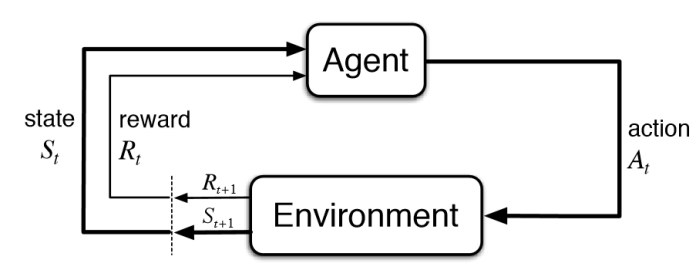
\includegraphics[width=1\textwidth]{figures/rl_general.jpg}
	\caption{Reinforcement Learning. An agent chooses an action to interact with the environment and gets a reward and an observation of his new state back. %todo\cite{rl_general.jpg}
		}
\end{figure}

%TODO exploration vs exploitation ? epsilon-greedy, soft min max

%%neuronal networks
\section{Artificial Neural Networks}

Artificial Neural Networks are inspired by the human brain. 
%\nnbio, blablabla
The Neural Network consists of layers of neurons. Each neuron is connected to the next layer of neurons. There is one input layer and one output layer at the beginning and end of the layer of neurons. The layers between the input and output layers are called hidden layer. The hidden layer can consist of only one or more layers. The idea is to train the neural network to take inputs and produce outputs. To approximate the value functions the input would be states and actions, the output should be the correct and optimal value of these states and actions. An example of an artificial neural network is shown in Figure 2.2.

\begin{figure} [h]
	
	\centering
	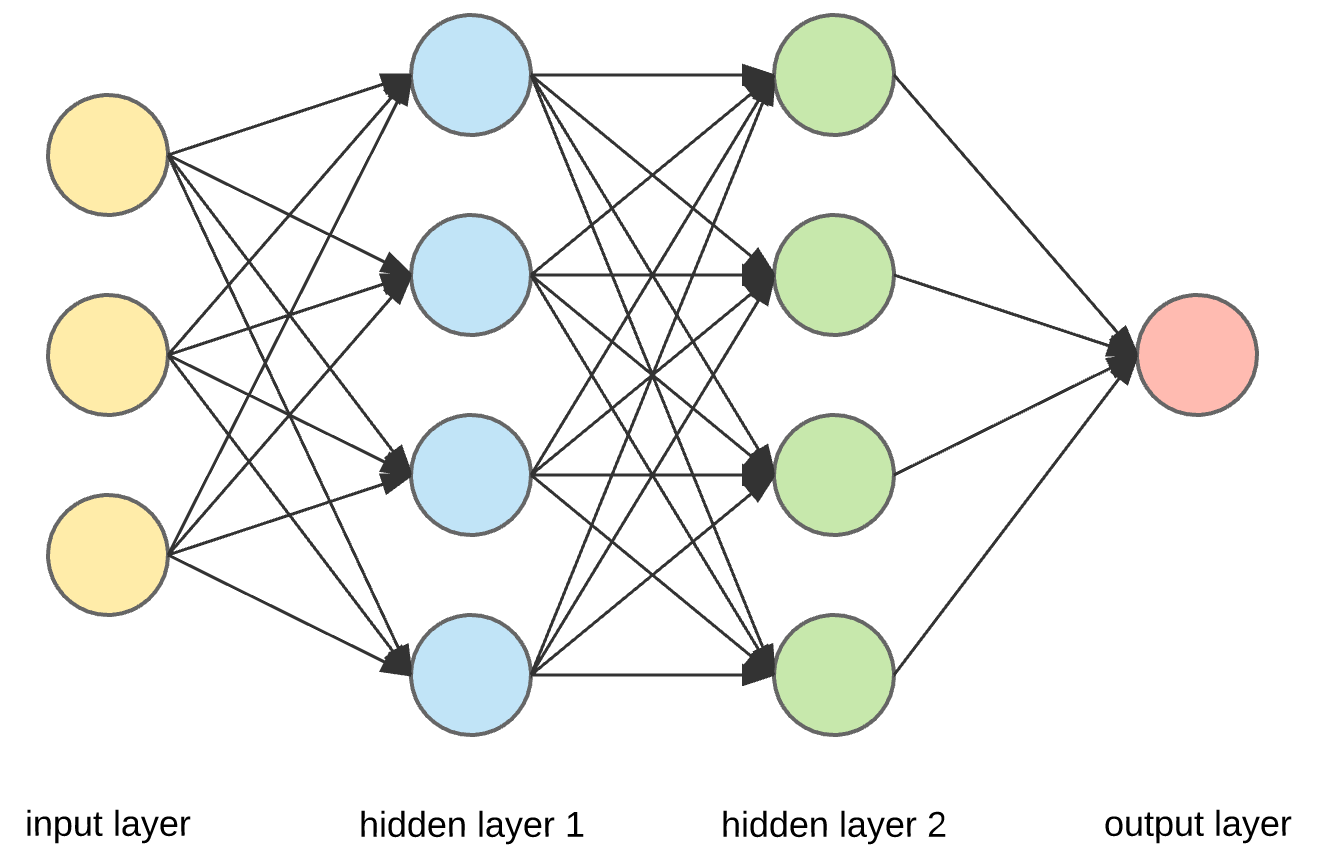
\includegraphics[width=1\textwidth]{figures/neural_network.png}
	\caption{A neural network. %todo\cite{neural_network.png}
	}
\end{figure}

\vspace{0.5cm}

The learning process of the neuronal network is as follows. Each neuron obtains inputs xi by the the output of the neurons in the layer before it. each input value is weighed and then added. A bias b is also added to support the learning process. After using an activation function on the sum, the value is output to the next layer of neurons. The activation function is a simple function that either reduces the output of the neuron to 0 if the value is below a certain threshold, otherwise the value is output unfiltered.
The training process of the neuron can be seen in Figure 2.3.
%besser formulieren!

\begin{figure} [h]
	
	\centering
	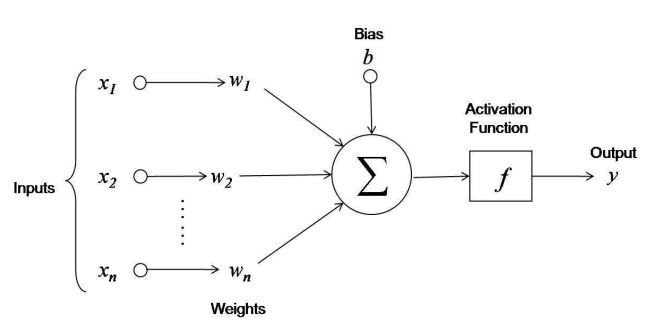
\includegraphics[width=1\textwidth]{figures/neuron.jpeg}
	\caption{A neuron. %todo\cite{neuron.jpeg}
	}
\end{figure}

When the neural network outputs a value, a process called Backpropagation is used to further improve the neural network.
%TODO Backpropagation
 

\vspace{0.5cm}



\section{Deep Deterministic Policy Gradients}

The algorithm Deep Deterministic Policy Gradient learns concurrently a Q-function (the action-value function) and a policy.
%TODO \ddpg
When learning the optimal action value function Q*(s,a), the optimal action in each state can be solved by using following equation:

%TODO insert ddpg equation 1

To solve the equations for a discrete action space, the Q-values of each action could be calculated and compared to find the biggest value. But in a continuous action space it is not possible to calculate the Q-value for each action. DDPG uses the fact that the action space is continuous and so Q*(s,a) is expected to be differentiable in respect to the action argument. %\cite{(ddpg)}
This way it is possible to approximate the Q-values and policy.


To learn the Q-values, the Bellman equation for the action value is used. To approximate the Q-values, a mean squared Bellman error function is used:

%TODO explain parameters better, do equation MSBE ddpg

Minimizing the MSBE loss function is equal to approximating the current Q-values to the optimal Q-values.

\vspace{0.5cm}

For DDPG an experience replay buffer is also used. The replay buffer is a set of experiences. This can be used to replay old experiences. When only using new experiences, the neural network might be overfitted to those experiences. Experience replay is useful to prevent that. But a too large buffer can cause the learning process to slow down. The right balance has to be found.

DDPG also uses target networks. The following term is called target:
%TODO add term
When minimizing the MSBE loss function, there is the problem that the target is also dependent on the parameters that are trained. When changing the parameters, the target would also change which is problematic. That is why the target network, a cpoy of the neural network is used. The update of the target network is delayed to avoid this conflict.

\vspace{0.5cm}

To find the optimal policy, simply gradient ascent can be used to find the maximal Q-values.

%pseudocode ?




\section{Hindsight Experience Replay}

%subsection curriculum learning ?

%read paper, use it

Sparse rewards are a big issue in Reinforcement Learning, especially in tasks for robotic arms often the rewards are sparse. Having sparse rewards means that most of the samples used for training will not successful and therefore will not bring any useful reward. For example, the task to move an object to a certain point would have a sparse reward for a robotic arm because very precise movements are needed which the robotic arm has to learn first.
 
\vspace{0.5cm}
 
Andrychowicz et al. have shown that Hindsight Experience Replay can be used to deal with this issue for robotic arms. 
%TODO \herpaper
Hindsight Experience Replay can learn efficiently from sparse rewards and can also be combined with any off-policy Reinforcement Learning algorithm.
%TODO explain off-policy in rl chapter
This technique is inspired by the ability of humans to learn from failures as least as much as from successes.

\vspace{0.5cm}

Hindsight Experience Replay works as follows. After an episode of gaining experiences, all transitions between the states in each training sample is stored in a replay buffer, but the goal that was not achieved is extended to a set with a goal that is reached. This can also be further extended to a set of more goals that can be achieved in the terminating state of the training sample. If the goal was to move an object to point x, but it was pushed to point y, the replay buffer would use the same transitions but change the the goal we wanted to achieve to y. So when replaying the same experience, the agent would be successful and earn an useful reward. This does not help the agent learn how to reach the goal it wanted to reach initially, but it learns to reach other goals. Reaching those other achieved goals might be beneficial in learning how to reach the goal it actually wanted to achieve. Hindsight Experience Replay is mainly used for tasks with multiple goals, but it was shown that it also improves the training of tasks with only a single goal. 
%TODO ref herpaper 
Interestingly, they have shown Hindsight Experience Replay performs has problems when using shaped rewards
%add binary rewards at start of section ?. binary != shaped ?
 
 %add pseudocode ?



\section{Hindsight Goal Generation*}

%read paper, use it

%delete ?